% Created by tikzDevice version 0.12.3.1 on 2022-12-09 10:51:37
% !TEX encoding = UTF-8 Unicode
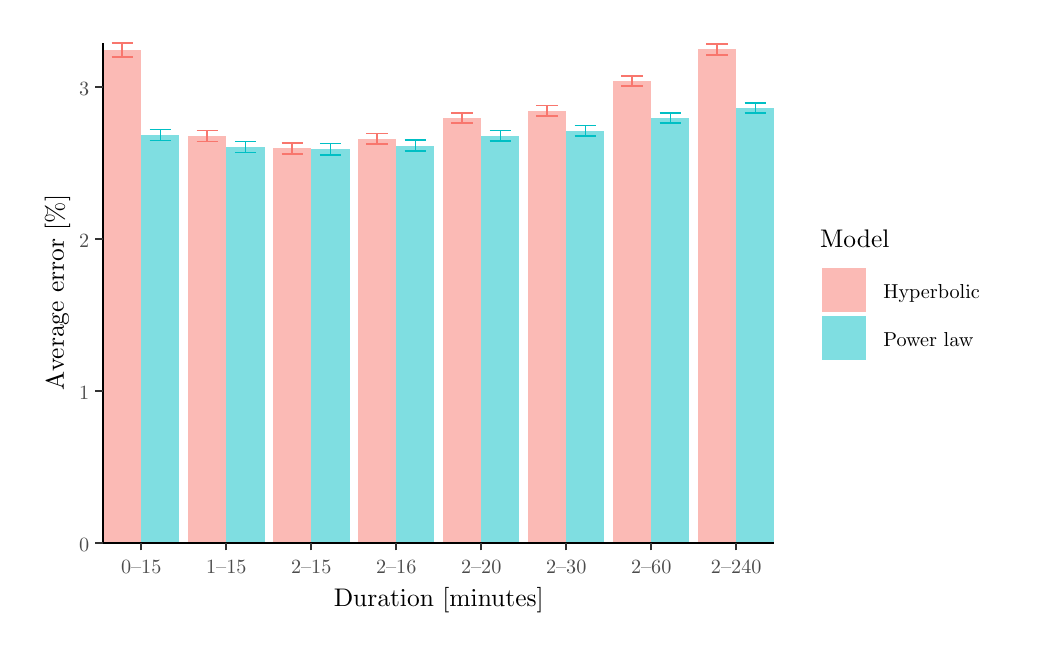
\begin{tikzpicture}[x=1pt,y=1pt]
\definecolor{fillColor}{RGB}{255,255,255}
\path[use as bounding box,fill=fillColor,fill opacity=0.00] (0,0) rectangle (361.35,216.81);
\begin{scope}
\path[clip] (  0.00,  0.00) rectangle (361.35,216.81);
\definecolor{drawColor}{RGB}{255,255,255}
\definecolor{fillColor}{RGB}{255,255,255}

\path[draw=drawColor,line width= 0.6pt,line join=round,line cap=round,fill=fillColor] (  0.00,  0.00) rectangle (361.35,216.81);
\end{scope}
\begin{scope}
\path[clip] ( 27.22, 30.69) rectangle (269.85,211.31);
\definecolor{fillColor}{RGB}{255,255,255}

\path[fill=fillColor] ( 27.22, 30.69) rectangle (269.85,211.31);
\definecolor{fillColor}{RGB}{248,118,109}

\path[fill=fillColor,fill opacity=0.50] ( 27.22, 30.69) rectangle ( 41.04,208.74);
\definecolor{fillColor}{RGB}{0,191,196}

\path[fill=fillColor,fill opacity=0.50] ( 41.04, 30.69) rectangle ( 54.86,177.99);
\definecolor{fillColor}{RGB}{248,118,109}

\path[fill=fillColor,fill opacity=0.50] ( 57.93, 30.69) rectangle ( 71.76,177.63);
\definecolor{fillColor}{RGB}{0,191,196}

\path[fill=fillColor,fill opacity=0.50] ( 71.76, 30.69) rectangle ( 85.58,173.72);
\definecolor{fillColor}{RGB}{248,118,109}

\path[fill=fillColor,fill opacity=0.50] ( 88.65, 30.69) rectangle (102.47,173.22);
\definecolor{fillColor}{RGB}{0,191,196}

\path[fill=fillColor,fill opacity=0.50] (102.47, 30.69) rectangle (116.29,172.91);
\definecolor{fillColor}{RGB}{248,118,109}

\path[fill=fillColor,fill opacity=0.50] (119.36, 30.69) rectangle (133.18,176.61);
\definecolor{fillColor}{RGB}{0,191,196}

\path[fill=fillColor,fill opacity=0.50] (133.18, 30.69) rectangle (147.00,174.23);
\definecolor{fillColor}{RGB}{248,118,109}

\path[fill=fillColor,fill opacity=0.50] (150.07, 30.69) rectangle (163.89,184.09);
\definecolor{fillColor}{RGB}{0,191,196}

\path[fill=fillColor,fill opacity=0.50] (163.89, 30.69) rectangle (177.71,177.74);
\definecolor{fillColor}{RGB}{248,118,109}

\path[fill=fillColor,fill opacity=0.50] (180.78, 30.69) rectangle (194.61,186.83);
\definecolor{fillColor}{RGB}{0,191,196}

\path[fill=fillColor,fill opacity=0.50] (194.61, 30.69) rectangle (208.43,179.62);
\definecolor{fillColor}{RGB}{248,118,109}

\path[fill=fillColor,fill opacity=0.50] (211.50, 30.69) rectangle (225.32,197.57);
\definecolor{fillColor}{RGB}{0,191,196}

\path[fill=fillColor,fill opacity=0.50] (225.32, 30.69) rectangle (239.14,184.20);
\definecolor{fillColor}{RGB}{248,118,109}

\path[fill=fillColor,fill opacity=0.50] (242.21, 30.69) rectangle (256.03,208.96);
\definecolor{fillColor}{RGB}{0,191,196}

\path[fill=fillColor,fill opacity=0.50] (256.03, 30.69) rectangle (269.85,187.87);
\definecolor{drawColor}{RGB}{248,118,109}

\path[draw=drawColor,line width= 0.6pt,line join=round] ( 30.29,211.31) --
	( 37.97,211.31);

\path[draw=drawColor,line width= 0.6pt,line join=round] ( 34.13,211.31) --
	( 34.13,206.16);

\path[draw=drawColor,line width= 0.6pt,line join=round] ( 30.29,206.16) --
	( 37.97,206.16);
\definecolor{drawColor}{RGB}{0,191,196}

\path[draw=drawColor,line width= 0.6pt,line join=round] ( 44.11,179.99) --
	( 51.79,179.99);

\path[draw=drawColor,line width= 0.6pt,line join=round] ( 47.95,179.99) --
	( 47.95,175.99);

\path[draw=drawColor,line width= 0.6pt,line join=round] ( 44.11,175.99) --
	( 51.79,175.99);
\definecolor{drawColor}{RGB}{248,118,109}

\path[draw=drawColor,line width= 0.6pt,line join=round] ( 61.01,179.61) --
	( 68.68,179.61);

\path[draw=drawColor,line width= 0.6pt,line join=round] ( 64.84,179.61) --
	( 64.84,175.64);

\path[draw=drawColor,line width= 0.6pt,line join=round] ( 61.01,175.64) --
	( 68.68,175.64);
\definecolor{drawColor}{RGB}{0,191,196}

\path[draw=drawColor,line width= 0.6pt,line join=round] ( 74.83,175.72) --
	( 82.50,175.72);

\path[draw=drawColor,line width= 0.6pt,line join=round] ( 78.67,175.72) --
	( 78.67,171.72);

\path[draw=drawColor,line width= 0.6pt,line join=round] ( 74.83,171.72) --
	( 82.50,171.72);
\definecolor{drawColor}{RGB}{248,118,109}

\path[draw=drawColor,line width= 0.6pt,line join=round] ( 91.72,175.24) --
	( 99.40,175.24);

\path[draw=drawColor,line width= 0.6pt,line join=round] ( 95.56,175.24) --
	( 95.56,171.21);

\path[draw=drawColor,line width= 0.6pt,line join=round] ( 91.72,171.21) --
	( 99.40,171.21);
\definecolor{drawColor}{RGB}{0,191,196}

\path[draw=drawColor,line width= 0.6pt,line join=round] (105.54,174.96) --
	(113.22,174.96);

\path[draw=drawColor,line width= 0.6pt,line join=round] (109.38,174.96) --
	(109.38,170.87);

\path[draw=drawColor,line width= 0.6pt,line join=round] (105.54,170.87) --
	(113.22,170.87);
\definecolor{drawColor}{RGB}{248,118,109}

\path[draw=drawColor,line width= 0.6pt,line join=round] (122.43,178.54) --
	(130.11,178.54);

\path[draw=drawColor,line width= 0.6pt,line join=round] (126.27,178.54) --
	(126.27,174.68);

\path[draw=drawColor,line width= 0.6pt,line join=round] (122.43,174.68) --
	(130.11,174.68);
\definecolor{drawColor}{RGB}{0,191,196}

\path[draw=drawColor,line width= 0.6pt,line join=round] (136.25,176.21) --
	(143.93,176.21);

\path[draw=drawColor,line width= 0.6pt,line join=round] (140.09,176.21) --
	(140.09,172.25);

\path[draw=drawColor,line width= 0.6pt,line join=round] (136.25,172.25) --
	(143.93,172.25);
\definecolor{drawColor}{RGB}{248,118,109}

\path[draw=drawColor,line width= 0.6pt,line join=round] (153.14,185.92) --
	(160.82,185.92);

\path[draw=drawColor,line width= 0.6pt,line join=round] (156.98,185.92) --
	(156.98,182.27);

\path[draw=drawColor,line width= 0.6pt,line join=round] (153.14,182.27) --
	(160.82,182.27);
\definecolor{drawColor}{RGB}{0,191,196}

\path[draw=drawColor,line width= 0.6pt,line join=round] (166.96,179.62) --
	(174.64,179.62);

\path[draw=drawColor,line width= 0.6pt,line join=round] (170.80,179.62) --
	(170.80,175.85);

\path[draw=drawColor,line width= 0.6pt,line join=round] (166.96,175.85) --
	(174.64,175.85);
\definecolor{drawColor}{RGB}{248,118,109}

\path[draw=drawColor,line width= 0.6pt,line join=round] (183.86,188.66) --
	(191.53,188.66);

\path[draw=drawColor,line width= 0.6pt,line join=round] (187.70,188.66) --
	(187.70,184.99);

\path[draw=drawColor,line width= 0.6pt,line join=round] (183.86,184.99) --
	(191.53,184.99);
\definecolor{drawColor}{RGB}{0,191,196}

\path[draw=drawColor,line width= 0.6pt,line join=round] (197.68,181.49) --
	(205.35,181.49);

\path[draw=drawColor,line width= 0.6pt,line join=round] (201.52,181.49) --
	(201.52,177.74);

\path[draw=drawColor,line width= 0.6pt,line join=round] (197.68,177.74) --
	(205.35,177.74);
\definecolor{drawColor}{RGB}{248,118,109}

\path[draw=drawColor,line width= 0.6pt,line join=round] (214.57,199.33) --
	(222.25,199.33);

\path[draw=drawColor,line width= 0.6pt,line join=round] (218.41,199.33) --
	(218.41,195.80);

\path[draw=drawColor,line width= 0.6pt,line join=round] (214.57,195.80) --
	(222.25,195.80);
\definecolor{drawColor}{RGB}{0,191,196}

\path[draw=drawColor,line width= 0.6pt,line join=round] (228.39,186.00) --
	(236.07,186.00);

\path[draw=drawColor,line width= 0.6pt,line join=round] (232.23,186.00) --
	(232.23,182.41);

\path[draw=drawColor,line width= 0.6pt,line join=round] (228.39,182.41) --
	(236.07,182.41);
\definecolor{drawColor}{RGB}{248,118,109}

\path[draw=drawColor,line width= 0.6pt,line join=round] (245.28,210.86) --
	(252.96,210.86);

\path[draw=drawColor,line width= 0.6pt,line join=round] (249.12,210.86) --
	(249.12,207.05);

\path[draw=drawColor,line width= 0.6pt,line join=round] (245.28,207.05) --
	(252.96,207.05);
\definecolor{drawColor}{RGB}{0,191,196}

\path[draw=drawColor,line width= 0.6pt,line join=round] (259.10,189.68) --
	(266.78,189.68);

\path[draw=drawColor,line width= 0.6pt,line join=round] (262.94,189.68) --
	(262.94,186.05);

\path[draw=drawColor,line width= 0.6pt,line join=round] (259.10,186.05) --
	(266.78,186.05);
\end{scope}
\begin{scope}
\path[clip] (  0.00,  0.00) rectangle (361.35,216.81);
\definecolor{drawColor}{RGB}{0,0,0}

\path[draw=drawColor,line width= 0.6pt,line join=round] ( 27.22, 30.69) --
	( 27.22,211.31);
\end{scope}
\begin{scope}
\path[clip] (  0.00,  0.00) rectangle (361.35,216.81);
\definecolor{drawColor}{gray}{0.30}

\node[text=drawColor,anchor=base east,inner sep=0pt, outer sep=0pt, scale=  0.73] at ( 22.27, 27.66) {0};

\node[text=drawColor,anchor=base east,inner sep=0pt, outer sep=0pt, scale=  0.73] at ( 22.27, 82.54) {1};

\node[text=drawColor,anchor=base east,inner sep=0pt, outer sep=0pt, scale=  0.73] at ( 22.27,137.43) {2};

\node[text=drawColor,anchor=base east,inner sep=0pt, outer sep=0pt, scale=  0.73] at ( 22.27,192.32) {3};
\end{scope}
\begin{scope}
\path[clip] (  0.00,  0.00) rectangle (361.35,216.81);
\definecolor{drawColor}{gray}{0.20}

\path[draw=drawColor,line width= 0.6pt,line join=round] ( 24.47, 30.69) --
	( 27.22, 30.69);

\path[draw=drawColor,line width= 0.6pt,line join=round] ( 24.47, 85.57) --
	( 27.22, 85.57);

\path[draw=drawColor,line width= 0.6pt,line join=round] ( 24.47,140.46) --
	( 27.22,140.46);

\path[draw=drawColor,line width= 0.6pt,line join=round] ( 24.47,195.35) --
	( 27.22,195.35);
\end{scope}
\begin{scope}
\path[clip] (  0.00,  0.00) rectangle (361.35,216.81);
\definecolor{drawColor}{RGB}{0,0,0}

\path[draw=drawColor,line width= 0.6pt,line join=round] ( 27.22, 30.69) --
	(269.85, 30.69);
\end{scope}
\begin{scope}
\path[clip] (  0.00,  0.00) rectangle (361.35,216.81);
\definecolor{drawColor}{gray}{0.20}

\path[draw=drawColor,line width= 0.6pt,line join=round] ( 41.04, 27.94) --
	( 41.04, 30.69);

\path[draw=drawColor,line width= 0.6pt,line join=round] ( 71.76, 27.94) --
	( 71.76, 30.69);

\path[draw=drawColor,line width= 0.6pt,line join=round] (102.47, 27.94) --
	(102.47, 30.69);

\path[draw=drawColor,line width= 0.6pt,line join=round] (133.18, 27.94) --
	(133.18, 30.69);

\path[draw=drawColor,line width= 0.6pt,line join=round] (163.89, 27.94) --
	(163.89, 30.69);

\path[draw=drawColor,line width= 0.6pt,line join=round] (194.61, 27.94) --
	(194.61, 30.69);

\path[draw=drawColor,line width= 0.6pt,line join=round] (225.32, 27.94) --
	(225.32, 30.69);

\path[draw=drawColor,line width= 0.6pt,line join=round] (256.03, 27.94) --
	(256.03, 30.69);
\end{scope}
\begin{scope}
\path[clip] (  0.00,  0.00) rectangle (361.35,216.81);
\definecolor{drawColor}{gray}{0.30}

\node[text=drawColor,anchor=base,inner sep=0pt, outer sep=0pt, scale=  0.73] at ( 41.04, 19.68) {0--15};

\node[text=drawColor,anchor=base,inner sep=0pt, outer sep=0pt, scale=  0.73] at ( 71.76, 19.68) {1--15};

\node[text=drawColor,anchor=base,inner sep=0pt, outer sep=0pt, scale=  0.73] at (102.47, 19.68) {2--15};

\node[text=drawColor,anchor=base,inner sep=0pt, outer sep=0pt, scale=  0.73] at (133.18, 19.68) {2--16};

\node[text=drawColor,anchor=base,inner sep=0pt, outer sep=0pt, scale=  0.73] at (163.89, 19.68) {2--20};

\node[text=drawColor,anchor=base,inner sep=0pt, outer sep=0pt, scale=  0.73] at (194.61, 19.68) {2--30};

\node[text=drawColor,anchor=base,inner sep=0pt, outer sep=0pt, scale=  0.73] at (225.32, 19.68) {2--60};

\node[text=drawColor,anchor=base,inner sep=0pt, outer sep=0pt, scale=  0.73] at (256.03, 19.68) {2--240};
\end{scope}
\begin{scope}
\path[clip] (  0.00,  0.00) rectangle (361.35,216.81);
\definecolor{drawColor}{RGB}{0,0,0}

\node[text=drawColor,anchor=base,inner sep=0pt, outer sep=0pt, scale=  0.92] at (148.54,  7.64) {Duration [minutes]};
\end{scope}
\begin{scope}
\path[clip] (  0.00,  0.00) rectangle (361.35,216.81);
\definecolor{drawColor}{RGB}{0,0,0}

\node[text=drawColor,rotate= 90.00,anchor=base,inner sep=0pt, outer sep=0pt, scale=  0.92] at ( 13.08,121.00) {Average error [\%]};
\end{scope}
\begin{scope}
\path[clip] (  0.00,  0.00) rectangle (361.35,216.81);
\definecolor{fillColor}{RGB}{255,255,255}

\path[fill=fillColor] (280.85, 90.55) rectangle (355.85,151.45);
\end{scope}
\begin{scope}
\path[clip] (  0.00,  0.00) rectangle (361.35,216.81);
\definecolor{drawColor}{RGB}{0,0,0}

\node[text=drawColor,anchor=base west,inner sep=0pt, outer sep=0pt, scale=  0.92] at (286.35,137.30) {Model};
\end{scope}
\begin{scope}
\path[clip] (  0.00,  0.00) rectangle (361.35,216.81);
\definecolor{fillColor}{RGB}{248,118,109}

\path[fill=fillColor,fill opacity=0.50] (287.06,114.10) rectangle (302.98,130.02);
\end{scope}
\begin{scope}
\path[clip] (  0.00,  0.00) rectangle (361.35,216.81);
\definecolor{fillColor}{RGB}{0,191,196}

\path[fill=fillColor,fill opacity=0.50] (287.06, 96.76) rectangle (302.98,112.68);
\end{scope}
\begin{scope}
\path[clip] (  0.00,  0.00) rectangle (361.35,216.81);
\definecolor{drawColor}{RGB}{0,0,0}

\node[text=drawColor,anchor=base west,inner sep=0pt, outer sep=0pt, scale=  0.73] at (309.20,119.03) {Hyperbolic};
\end{scope}
\begin{scope}
\path[clip] (  0.00,  0.00) rectangle (361.35,216.81);
\definecolor{drawColor}{RGB}{0,0,0}

\node[text=drawColor,anchor=base west,inner sep=0pt, outer sep=0pt, scale=  0.73] at (309.20,101.69) {Power law};
\end{scope}
\end{tikzpicture}
